\documentclass[mathserif]{beamer}
\mode<presentation>
\usepackage{./simulabeamer}
\usepackage{./mymath}

\makeatletter % Let @ be a letter


%----------------------- Title and author ----------------------------
\title[Scientific Computing Seminar]{Adjoints}
\author{Simon W. Funke}
\institute{Simula Research Laboratory}
\date{\today}
\makeatother
\color{black}
%------------------------ Document start -----------------------------
\begin{document}
\simulatitlepage


\begin{frame}{Motivation}

\end{frame}


\begin{frame}{Algorithmic differentiation}
Given
\begin{equation}
f: \mathbb R^n \to \mathbb R^m, x \mapsto y
\end{equation}
Goal: Compute
\begin{equation}
\frac{\partial f}{\partial x} = \left(\frac{\partial f_i}{\partial x_j}\right)_{i, j}
\end{equation}
\end{frame}

%------------------------ Motivation ---------------------------------
\begin{frame}{What is an adjoint model?}
  

In the machine learning community it is called \emph{back-propagation}.

\end{frame}



%------------------------ Motivation ---------------------------------
\begin{frame}{Why is it useful?}
  

\end{frame}


% %------------------------ Motivation ---------------------------------
% \begin{frame}{Motivation - Rotating tidal-turbines\section{Motivation}}
%   \begin{figure}
%     \centering
%     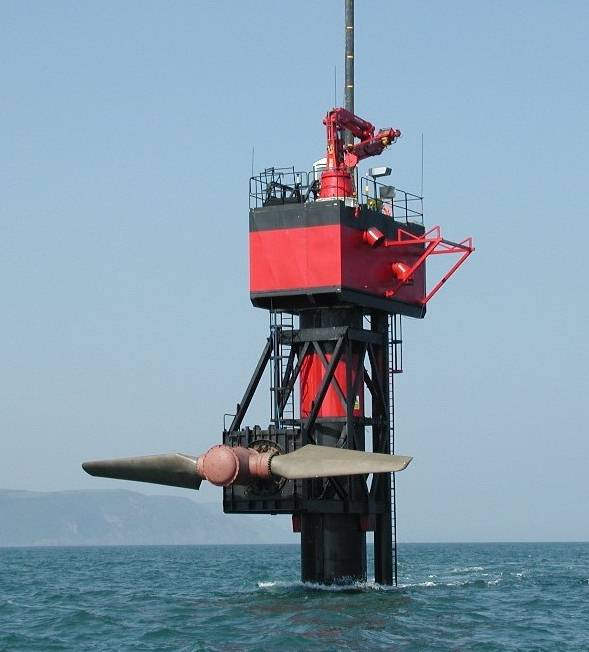
\includegraphics[width=0.5\textwidth]{media/seaflow.jpg}
%     \caption{The Tidal-stream turbine named Seaflow.}
%   \end{figure}
% \end{frame}

% \begin{frame}{Motivation -  General optimization problem}
%   \begin{itemize}
%   \item Optimization problems with PDE's as constraint
%     \begin{align}
%       \min_{u,m}\quad&J(u,m),\\
%       \text{subject to  } & F(u,m)=0
%     \end{align}
%   \item Costly to solve PDE
%     \begin{itemize}
%     \item Gradient Based Optimization
%     \end{itemize}
%   \item One functional of interest, large number of design parameters
%     \begin{itemize}
%     \item Adjoint Equations
%     \end{itemize}

%   \end{itemize}

  
% \end{frame}

% \begin{frame}{Representation of Dynamical Domains}
%   \begin{columns}
%     \column{0.5\linewidth}
%     \begin{figure}
%       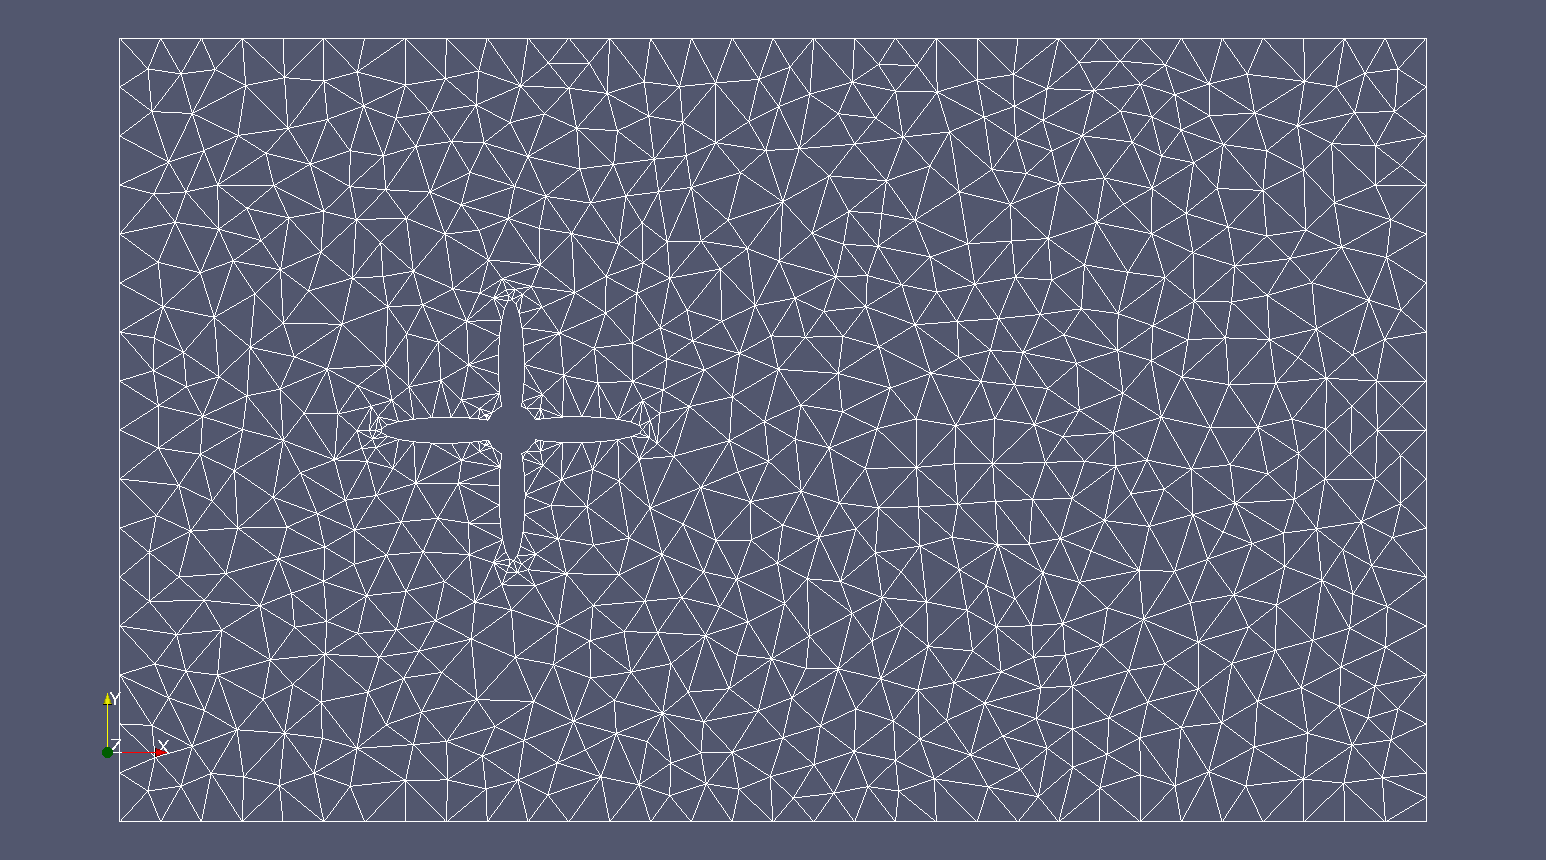
\includegraphics[width=\linewidth]{media/singlemesh.png}
%       %% \caption{\href{file:///home/dokken/Documents/Simula/ChalmersOkt/Presentation/singlemovie.avi}
%       \caption{\href{./media/singlemovie.avi}{Turbine rotating with prescribed velocity with smoothing of mesh movements}}
      
%     \end{figure}

%     \column{0.5\linewidth}
%     \begin{figure}
%       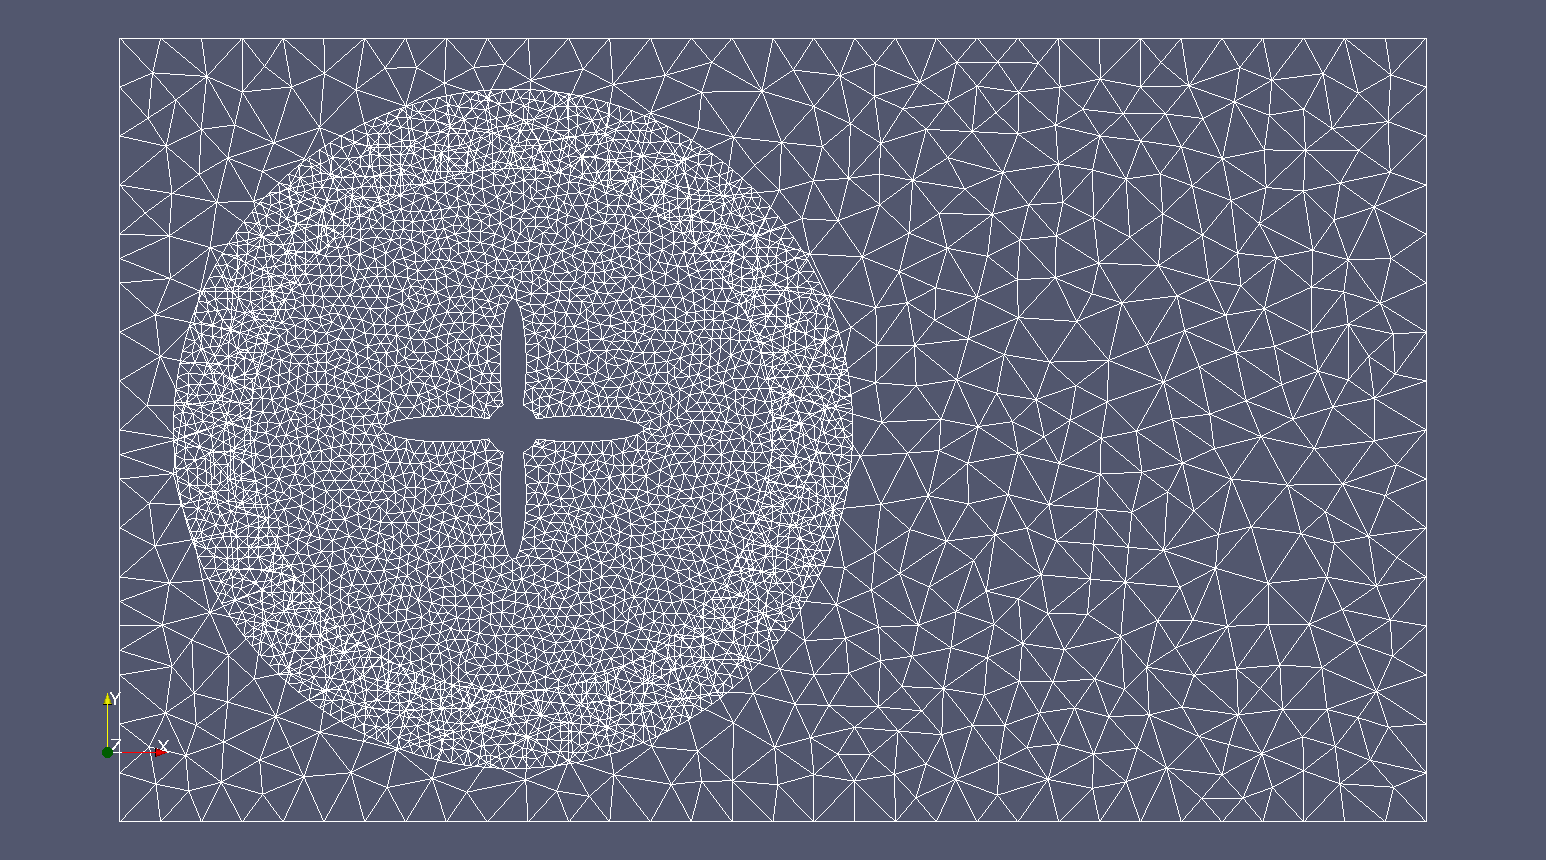
\includegraphics[width=\linewidth]{media/multimesh.png}
%       %% \caption{\href{file:///home/dokken/Documents/Simula/ChalmersOkt/Presentation/multimovie.avi}{Turbine rotating with prescribed velocity with overlapping meshes}}
%       \caption{\href{./media/multimovie.avi}{Turbine rotating with prescribed velocity with overlapping meshes}}
%     \end{figure}
%   \end{columns}
  
  
% \end{frame}
 
% \begin{frame}{Overlapping meshes\section{Overlapping meshes}}
%   \begin{columns}
%     \column{0.5\linewidth}
%     \textbf{Our approach}
%     \begin{itemize}
%     \item Nitsche method for interface conditions on the boundary of meshes meshes 
%     \end{itemize}
%     \textbf{Challenge}
%     \begin{itemize}
%     \item Detect where the two meshes intersect
%     \end{itemize}
%     \column{0.5\linewidth}
%     \begin{figure}
%       \centering
%       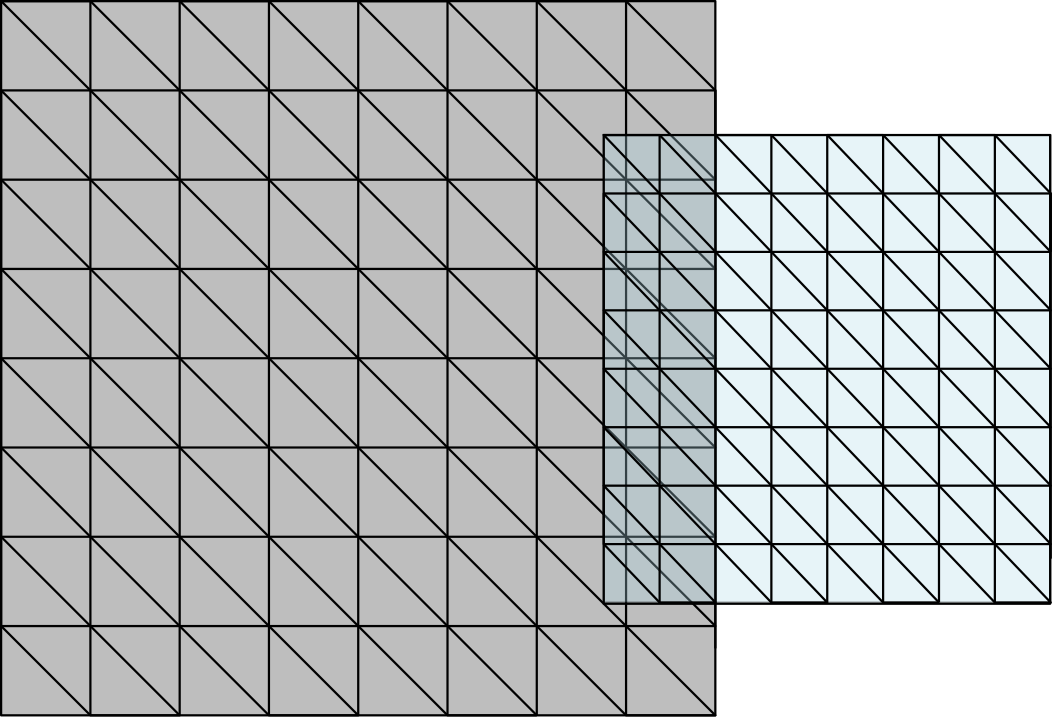
\includegraphics[width=\linewidth]{media/overlapmesh.png}
%       \caption{Illustration of overlapping meshes.}
%     \end{figure}
%   \end{columns}
% \end{frame}


% \begin{frame}{Coupling between overlapping domains and meshes}
%   \begin{figure}
%     \centering
%     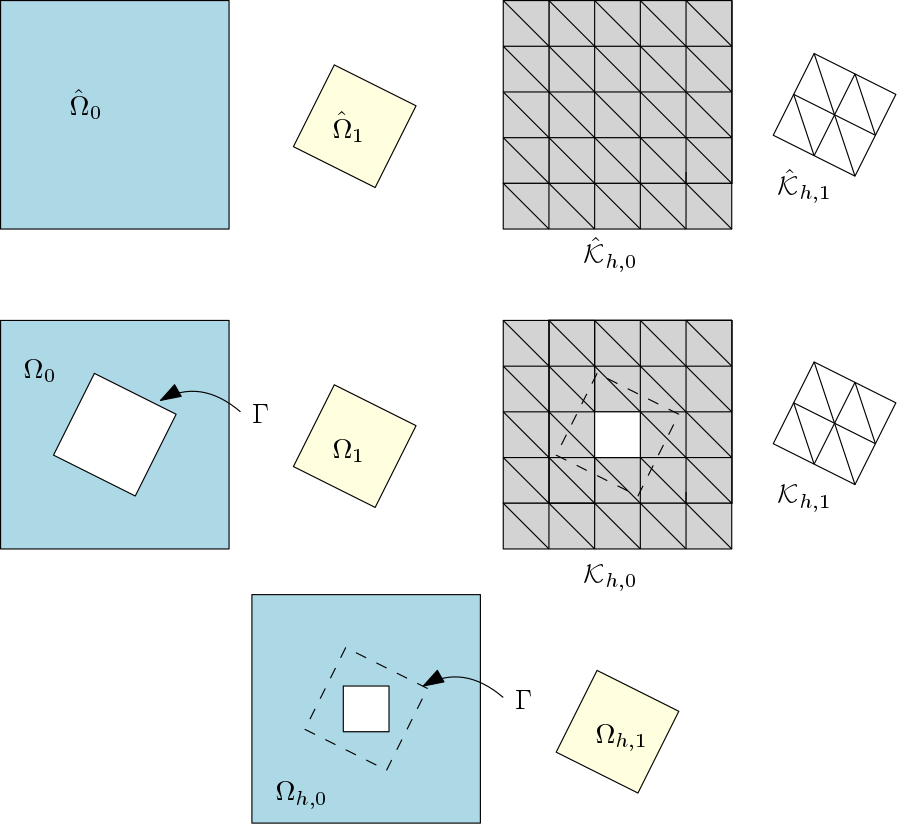
\includegraphics[width=0.6\linewidth]{media/domain_mesh.png}
%     \caption{How to create a computational domain for two meshes.}
%   \end{figure} 
% \end{frame}

% \begin{frame}{Heat-equation with Backward Euler in time}
%   \begin{columns}
%     \column{0.65\linewidth}
%     \textbf{Discretization in time and interface-conditions}
%     \begin{align*}
%       \frac{u^n-u^{n-1}}{\Delta t} - \nabla^2 u^n&= f(t^n)
%       \quad \text{in}\quad \Omega_0\cup\Omega_1\\
%             [\![u^n]\!]&=0\\
%             [\![\mathbf n \cdot \nabla u^n]\!]&=0
%     \end{align*}
%     \textbf{Notation}
%     \begin{align*}
%       u^n&=(u^n_{\Omega_0},u^n_{\Omega_1})\\
%       [\![v]\!]&=v_0\vert_\Gamma-v_1\vert_\Gamma\\
%       \langle v \rangle &= \frac{v_0+v_1}{2} 
%     \end{align*}

%     \column{0.35\linewidth}
%     \begin{figure}
%       \centering
%       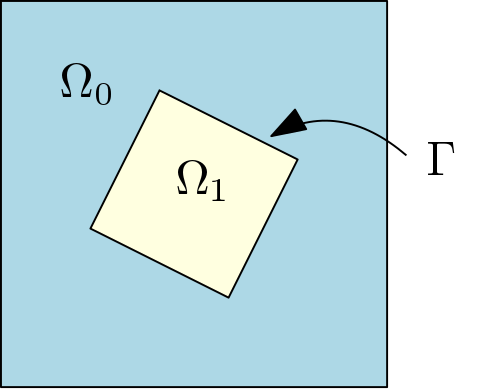
\includegraphics[width=\linewidth]{media/domains.png}
%       \caption{Domain of interest.}
%     \end{figure}
%   \end{columns}
% \end{frame}

% \begin{frame}{Variational form of the problem using Nitsches method
%     \section{Nitsches method}}
%   \begin{itemize}
%   \item Modify the standard variational form by \text{\color{red}integration
%     of the jump-condition for $u$ on $\Gamma$}.\\
%   \item For \text{\color{blue}symmetry} and
%     \text{\color{teal}coercivity} two extra terms are also added.
%   \end{itemize}
%   \begin{align*}
%   a_h(U^n,v)&=L(v), \quad \forall v\in V^h,\\
%   a_h(U^n,v):&=\sum_{i=1}^2\Big( (\nabla U_i^n, \nabla v_i)_{\Omega_i}+
%   \frac{1}{\Delta t}(U_i^n, v_i)_{\Omega_i}\Big)\\
%   &- \mathbin{\textcolor{red}{([\![U^n]\!], \langle\mathbf{n}\cdot\nabla v_h\rangle)_\Gamma}}
%   - \mathbin{\textcolor{blue}{([\![ v^h]\!], \langle\mathbf{n}\cdot\nabla U^n\rangle)_\Gamma}}\\
%   &+\mathbin{\textcolor{teal}{ (\gamma h^{-1} [\![U^n]\!], [\![v]\!])_\Gamma\nonumber}},\\
%   L(v)&=\sum_{i=1}^2\left((f,v_i)_{\Omega_i}+\frac{1}{\Delta t}(U_i^{n-1},v_i)_{\Omega_i} \right).
% \end{align*}
% \end{frame}

% \begin{frame}{Adjoint equations\section{Adjoint equations}}
%   \textbf{Optimization problem}
%   \begin{columns}
%     \column{0.5\linewidth}
%     \begin{align*}
%       \min_{u,m}\quad&J(u,m),\\
%       \text{subject to  } & F(u,m)=0
%     \end{align*}
%     \textbf{Reduced Functional}
%     \begin{align*}
%       \hat J(m)=J(u(m),m)
%     \end{align*}
%     \textbf{Gradient of Functional}
%     \begin{align*}
%       \totder{J}{m}=\der{J}{u}\totder{u}{m}+\der{J}{m}
%     \end{align*}
    
%     \column{0.5\linewidth}
%     \begin{itemize}
%     \item One goal-functional $J$.\vspace{0.5cm}
%     \item Large number of design-parameters $m$.\vspace{0.5cm}
%     \item Evaluation in the space of the design parameter is costly.\vspace{0.5cm}
%     \item Gradient-based optimization
%     \end{itemize}
%   \end{columns}
% \end{frame}

% \begin{frame}{The Adjoint equation}
%   \begin{align}
%     &\textbf{Gradient of Functional}\nonumber\\  
%     &\totder{J}{m}=\der{J}{u}\totder{u}{m}+\der{J}{m}\nonumber\\
%     &\textbf{Rewriting the gradient of the functional}\nonumber\\
%     &\left(\totder{J}{m}\right)^*=\left(\der{F}{m}\right)^*
%     \lambda+\left(\der{J}{m}\right)^*\nonumber\\
%     &\textbf{The adjoint equation}\nonumber\\
%     &\left(\der{F}{u} \right)^*\lambda = \der{J}{u}^*\label{adjoint}
%   \end{align}
  
%   \begin{itemize}
%   \item Avoid computation of Jacobian by using the adjoint method
%   \item Solving Equation (\ref{adjoint}) require 
%     specification of functional, not of design parameter.
%   \end{itemize}

% \end{frame}

% \begin{frame}{FEniCS and dolfin-adjoint\section[Applications]{Applications in FEniCS with dolfin-adjoint}}
%   \begin{figure}
%     
\includegraphics[height=0.15\textheight,left]{media/fenics.png}
%   \end{figure}
%   \begin{itemize}
%   \item Software for solving PDEs
%   \item \textbf{MultiMesh} - Implementation of overlapping meshes
%   \end{itemize}
%   \begin{figure}
%     
\includegraphics[height=0.15\textheight,left]{media/dolfin_adjoint.png}
%   \end{figure}
%   \begin{itemize}
%   \item Automatic derivation of the adjoint equations
%   \end{itemize}
% \end{frame}

% \begin{frame}{Optimal Poisson problem\section[Results]{Results}}
%   Finding the best heating/cooling $f$ of a cook-top to get a
%   desired temperature profile $d$.
%   \begin{align*}
%     \min_{u,f}J(u(f),f))&=\min_{u,f}\left(\half\Int{\Omega}{}(u-d)^2\md\Omega
%     + \frac{\alpha}{2}\Int{\Omega}{}f^2\md\Omega\right)\\
%     \text{subject to}&
%     \begin{cases}
%       -\nabla^2 u &= f\qquad \text{in }\Omega\\
%       u&=0 \qquad\text{on }\partial\Omega\\
%     \end{cases}
%   \end{align*}
%   Given a desired temperature profile
%   \begin{align*}
%     d&=\frac{1}{2\pi^2}\sin(\pi x)\sin(\pi y),
%   \end{align*}
%   we have the analytical solution to the optimization problem
%   \begin{align*}
%     f &= \frac{\sin(\pi x)\sin(\pi y)}{1 + 4\alpha \pi^4}
%   \end{align*}

% \end{frame}

% \begin{frame}{Meshes used for the optimal Poisson problem}
%   \begin{columns}
%     \column{0.5\linewidth}
%     \begin{figure}
%       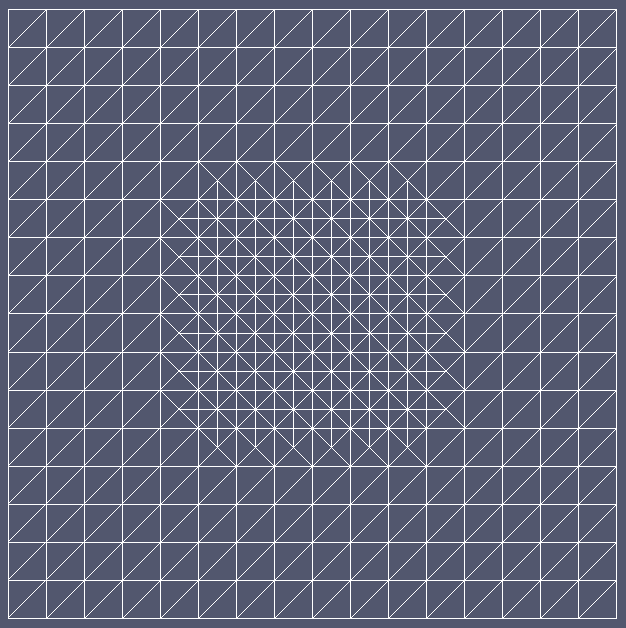
\includegraphics[width=\linewidth]{media/meshpoi.png}
%       \caption{Mesh used in dolfin for Optimization with a single mesh.}
%     \end{figure}
%     \column{0.5\linewidth}
%     \begin{figure}
%       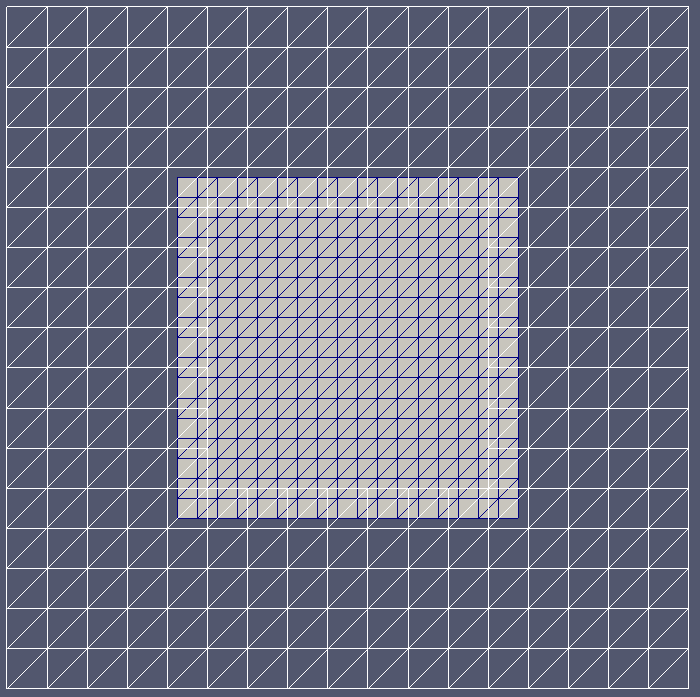
\includegraphics[width=\linewidth]{media/multimeshpoi.png}
%       \caption{MultiMesh used in dolfin for Optimization.}
%     \end{figure}
%   \end{columns}
% \end{frame}

% \begin{frame}{Results for Poisson-optimization}
%   \begin{columns}
%     \column{0.5\linewidth}
%     \begin{figure}
%       \centering
%       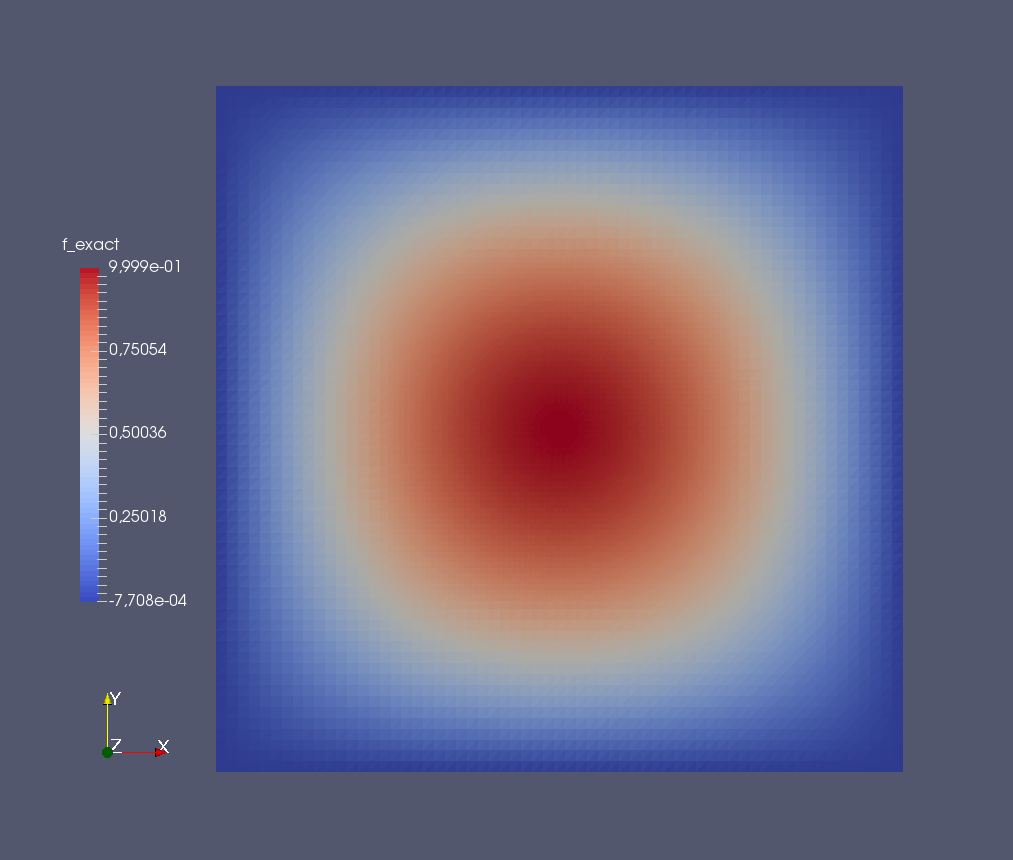
\includegraphics[width=\linewidth]{media/f_exact.png}
%       \caption{$f_{\text{analytical}}$ projected into a the same function-space as
%         the approximated solution (Piecewise constant functions).}
%     \end{figure}
%     \column{0.5\linewidth}
%     \begin{figure}
%       \centering
%       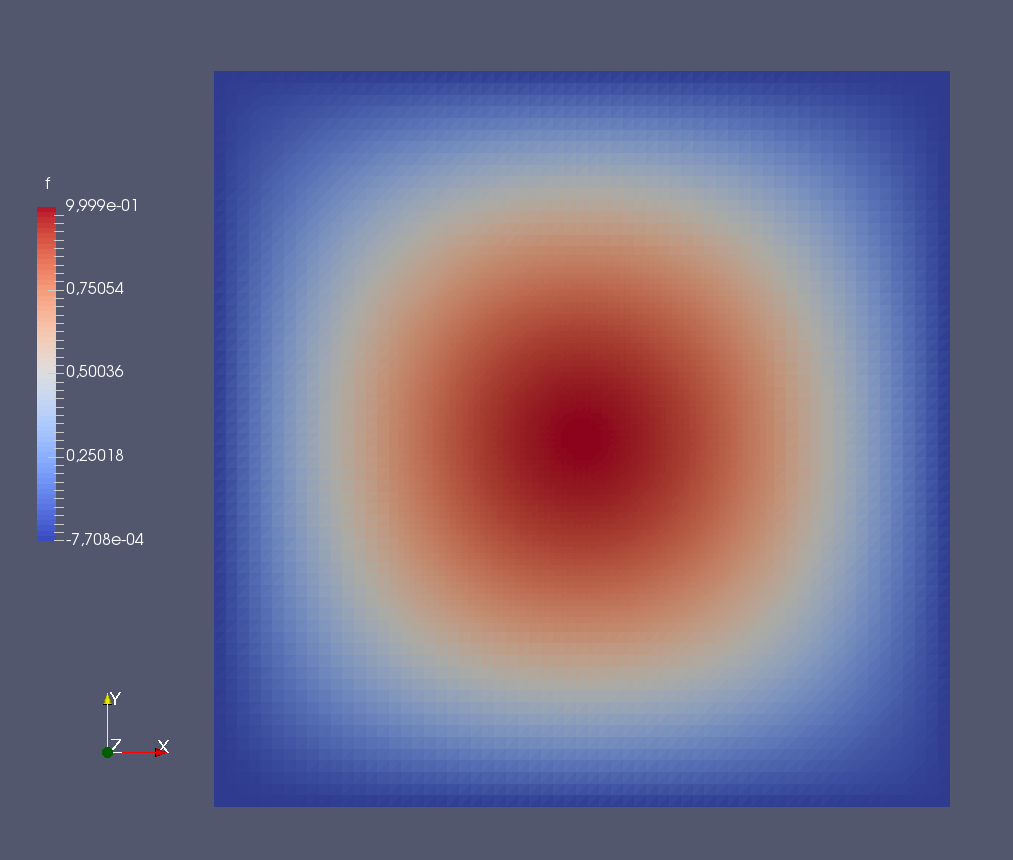
\includegraphics[width=\linewidth]{media/f_mm.png}
%       \caption{The resulting source-term $f$ for the optimization problem with MultiMesh where $f$ is approximated by piecewise constant functions.}
%     \end{figure}
%   \end{columns}
% \end{frame}


% \begin{frame}{Results for Poisson-optimization}
%   Computing the $L^2$-error of the computed $f$ and $u$.
%   \begin{figure}
%     \centering
%     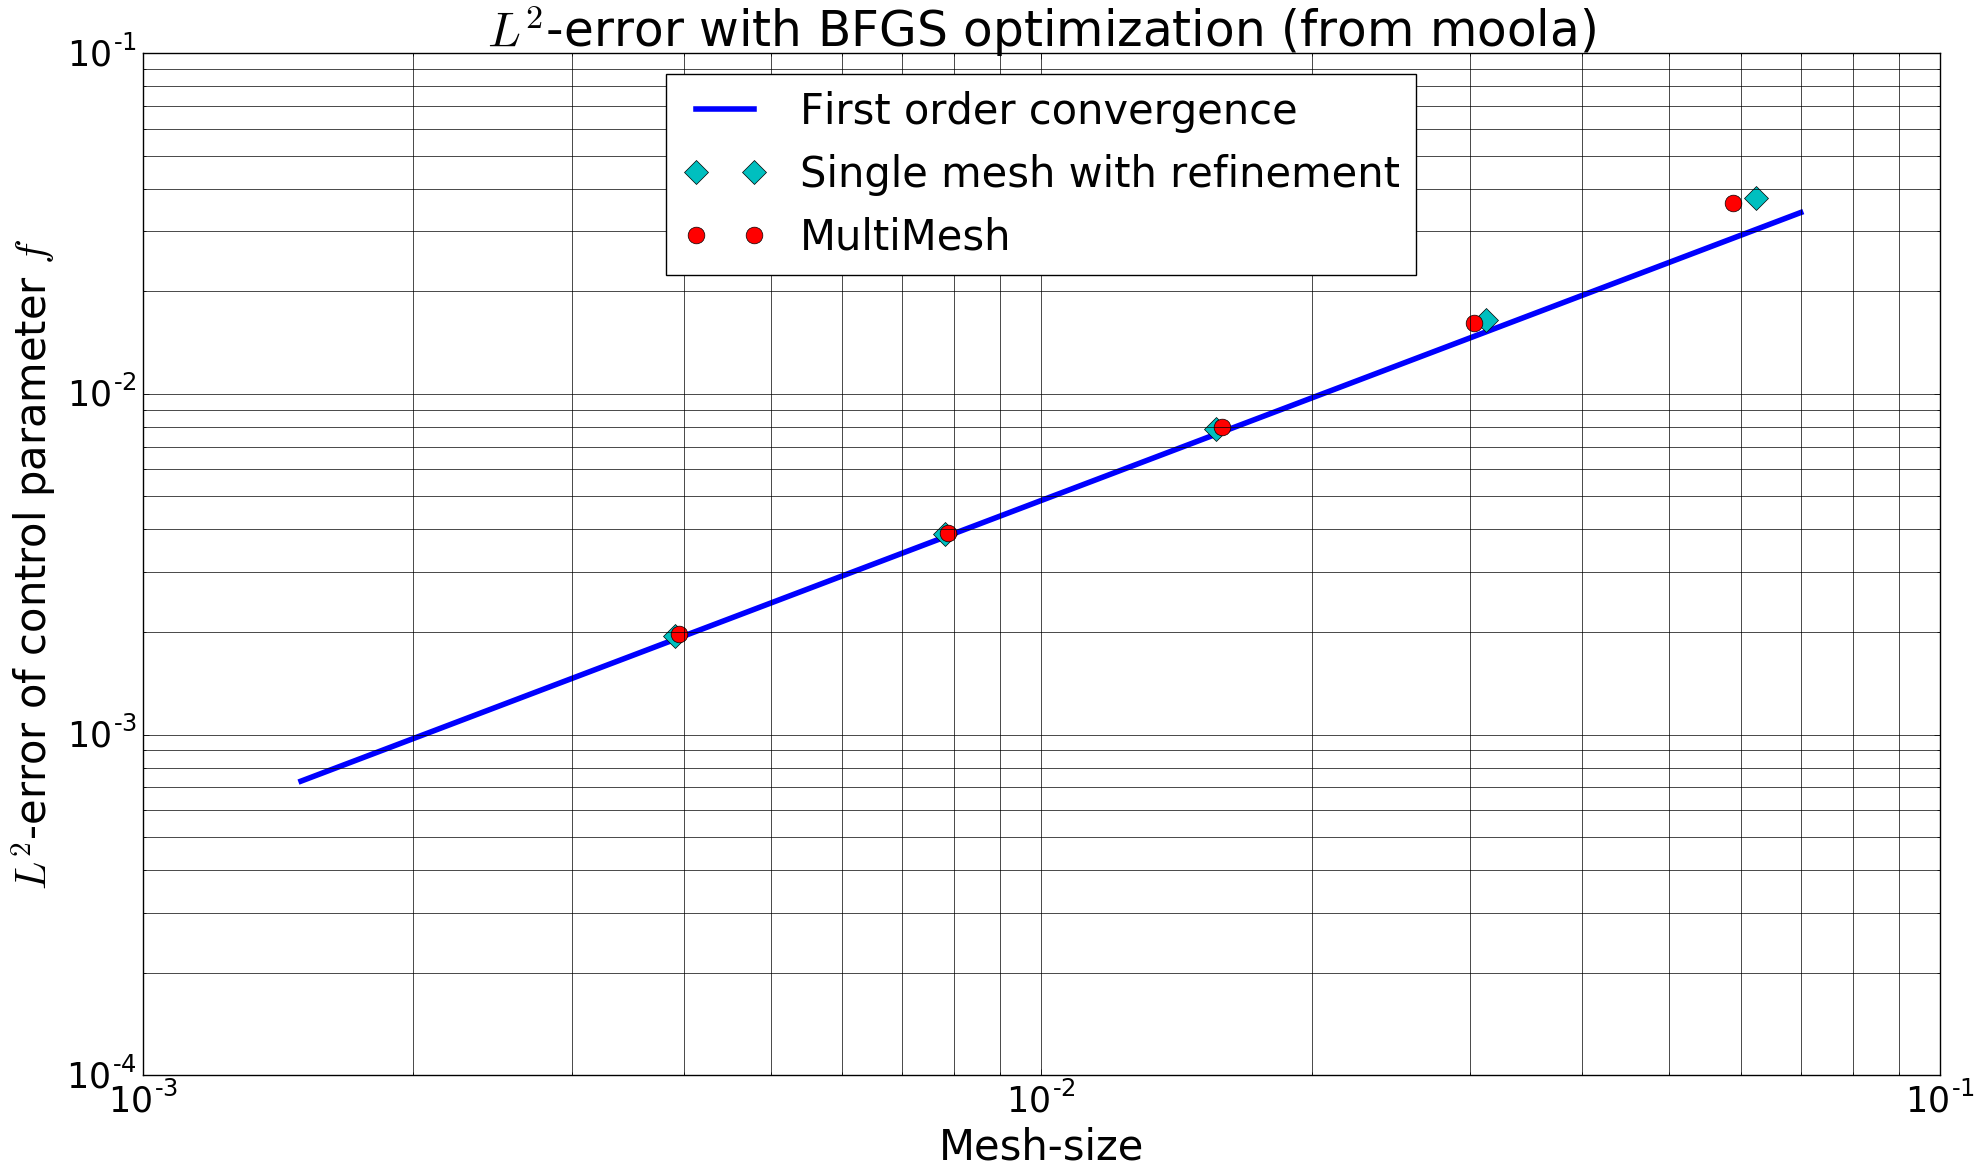
\includegraphics[width=0.9\linewidth]{media/L2control.png}
%     \caption{The error in the MultiMesh-problem is of the same size as the single mesh problem.}
%   \end{figure}
% \end{frame}

% \begin{frame}{Heat equation with moving domain}
%   \begin{figure}
%     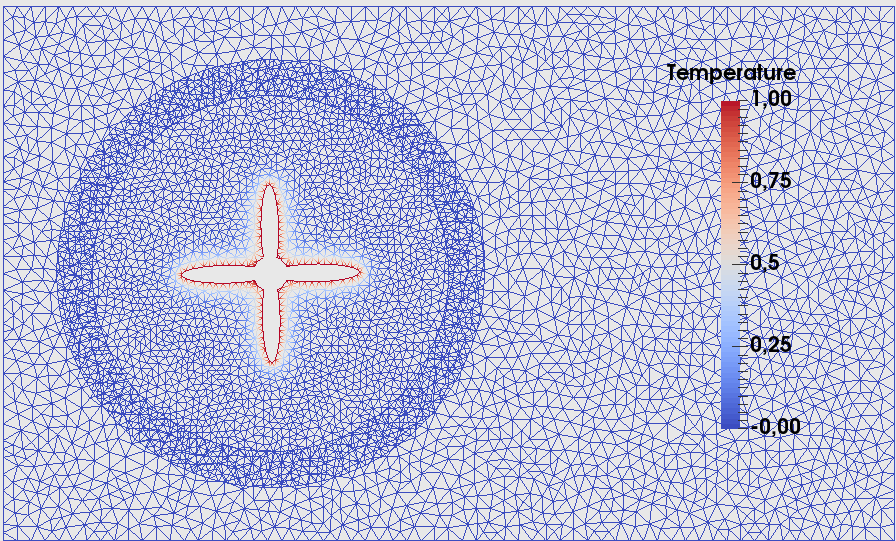
\includegraphics[width=0.8\linewidth]{media/heatsympic.png}
%     \caption{\href{./heatsym.avi}{Turbine rotating with prescribed velocity.}}
%        %% \caption{\href{file:///home/dokken/Documents/Simula/ChalmersOkt/Presentation/heatsym.avi}{Turbine rotating with prescribed velocity.}}
%   \end{figure}
% \end{frame}

% \begin{frame}{Investigation of the gradient of a goal functional}
%   \begin{align*}
%     \min_{u^0}&\hat{J}(u^0)=\Int{\Omega}{}\left(u^n(u^0)\right)^2\md\Omega,
%     \quad  u^0\text{ intital condtion,}\\
%     u^n&:\text{solution of the heat equation after n-timesteps.}
%   \end{align*}
%   \begin{figure}
%     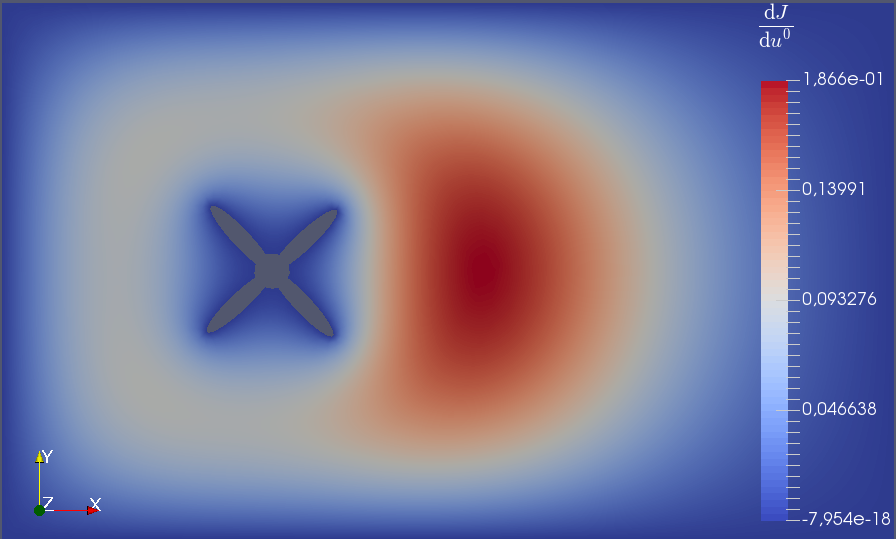
\includegraphics[width=0.6\linewidth]{media/dJdu0.png}
%     \caption{$\totder{J}{u^0}$ at time $T=1.5$. }
%   \end{figure}
% \end{frame}


% \begin{frame}{Further Work\section{Further Work}}
%   \begin{figure}
%     
\includegraphics[height=0.15\textheight,left]{media/forskningsradet.png}
%   \end{figure}
%   \begin{itemize}
%   \item \textbf{OptCutCell} - Extending dolfin-adjoint to use overlapping
%     domains and extending MultiMesh-user interface.
%   \end{itemize}
%   \begin{figure}
%     
\includegraphics[height=0.15\textheight,left]{media/opentidalfarm.jpg}
%     \begin{itemize}
%     \item Open-source optimization software for tidal turbine farms.
%     \item Optimal position of a set of dynamic tidal-stream turbines
%     \end{itemize}
%   \end{figure}
% \end{frame}
\end{document}
